\documentclass[pdftex,12pt,a4paper]{report}

\usepackage{amsmath}
\usepackage{amsfonts}
\usepackage{amssymb}

\usepackage[ngerman]{babel}
\usepackage[utf8]{inputenc}


\usepackage[pdftex]{graphicx}
\usepackage{wrapfig} % Paket zur Positionierung einbinden
\usepackage{listings}

% new commands
\newcommand{\HRule}{\rule{\linewidth}{0.5mm}}


\author{Nik\v{s}a Ra\v{s}i\'{c};Martin Weinberg}
\title{Proposal Projekt}

\begin{document}
\title{Projektproposal:}
\date{09.01.13}
\author{Nik\v{s}a Ra\v{s}i\'{c} \& Martin Weinberg}

\begin{titlepage}
\begin{center}
% Upper part of the page
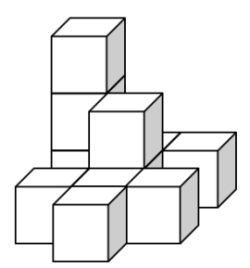
\includegraphics[width=0.4\textwidth]{./wuerfel}\\[1cm]    

\textsc{\LARGE Projektproposal}\\[1.5cm]

\textsc{\Large Creative Coding WS 12/13 }\\[0.5cm]


% Title
\HRule \\[0.4cm]
{ \huge \bfseries Emitting Cubes}\\[0.4cm]

\HRule \\[1.5cm]

% Author and supervisor
\begin{minipage}{0.4\textwidth}
\begin{flushleft} \large
\emph{Author:}\\
Nik\v{s}a Ra\v{s}i\'{c}  \&  \\ Martin Weinberg
\end{flushleft}
\end{minipage}
\begin{minipage}{0.4\textwidth}
\begin{flushright} \large
\emph{Supervisor:} \\ 
M. Sc.Alexander Neumann 
\end{flushright}
\end{minipage}

\vfill

% Bottom of the page
{\large \today}

\end{center}

\end{titlepage}

\tableofcontents
\newpage

\chapter{Emitting Cubes }
\section{Inspiration}
Im Rahmen mit der Veranstaltung Creative Coding hatten wir Berührung mit vielen Techniken zur kreativen Darstellung und Gestaltung. Eine davon ist Projektion Mapping, eine Technik die aus technischer Sicht sehr einfach umzusetzen ist, aber unglaublich viele Gestalterische Möglichkeiten bereit hält.Dabei werde Projektionsflächen per Software auf einem Objekt so "entzerrt" ,dass das Objekt  aussieht, als würde es von alle Seiten bestrahlt Es ist Allgemein bekannt wie dreidimensionale Objekte  auf zweidimensionale Flächen Projeziert werden können, der Umgekehrte Weg ist aber so ungewohnt und vielseitig einsetzbar, dass man sehr viele prägnante Möglichkeiten hat Werke zu erstellen. Diese Umstand hat uns so fasziniert, dass wir damit weiterarbeiten wollten. 

\section{Intention}
Wir wollten einmal mit der Technik des Projektion-Mappings arbeiten und sie einsetzten. Dabei sollte eine Konstruktion entstehen die sich durch ihre Besondere Darstellungsweise auszeichnet und wiederverwendet werden kann.

\section{Idee}
Im Rahmen unserer Silvesterfeier 2012/13 wollte wir eine ansprechendes Ambiente schaffen. Hierbei wollten wir der Dekoration unseren Touch geben und entschieden uns was eigenes zu bauen. Da in der Küche schon ein Beamer (FullHD) installiert ist wollten wir ihn in das Partykonzept einbinden. Somit war es nur ein kleiner Schritt zu den Würfeln. Grundidee war es Große Würfel zu bauen, die leicht schräg an die Decke montiert werden. Dadurch bietet jeder Würfel 3 Projektionsflächen die verschieden genutzt werden können. Am Ende waren es 3 Würfel mit insgesamt 9 Projektionsflächen. Dazu wurde eine Software geschrieben in Processing um die Flächen anzusteuern. Diese Flächen wurden während der gesamten Party angestrahlt. 2 davon zeigten Effekte , eine FFT am Line-Out sowie eine Lavalampe. Auf 3 zusammenhängenden Flächen wurde eine Countdown gezeigt, mit der Zeit bis zum Jahreswechsel, Auf den 4 größten Flächen wurden Bilder eingeblendet, die im Laufe des Abends geschossen wurden von der Party und von den Gästen. Da man bei solchen Partys nie mitbekommt wann geklingelt wurde, erweiterten wir die Software, mit einer WebCam und einem Tool zur Bewegungsdetektion an unserer Türklingel. Diese leuchtet immer wenn geklingelt wurde.  Als kleines Gimmick zeigten die Würfel mit einer kurzen Einblendung einer großen Glocke dann an, ob jemand geklingelt hat.


\section{Aufbau und Techniken}

\subsection{Die Würfel}

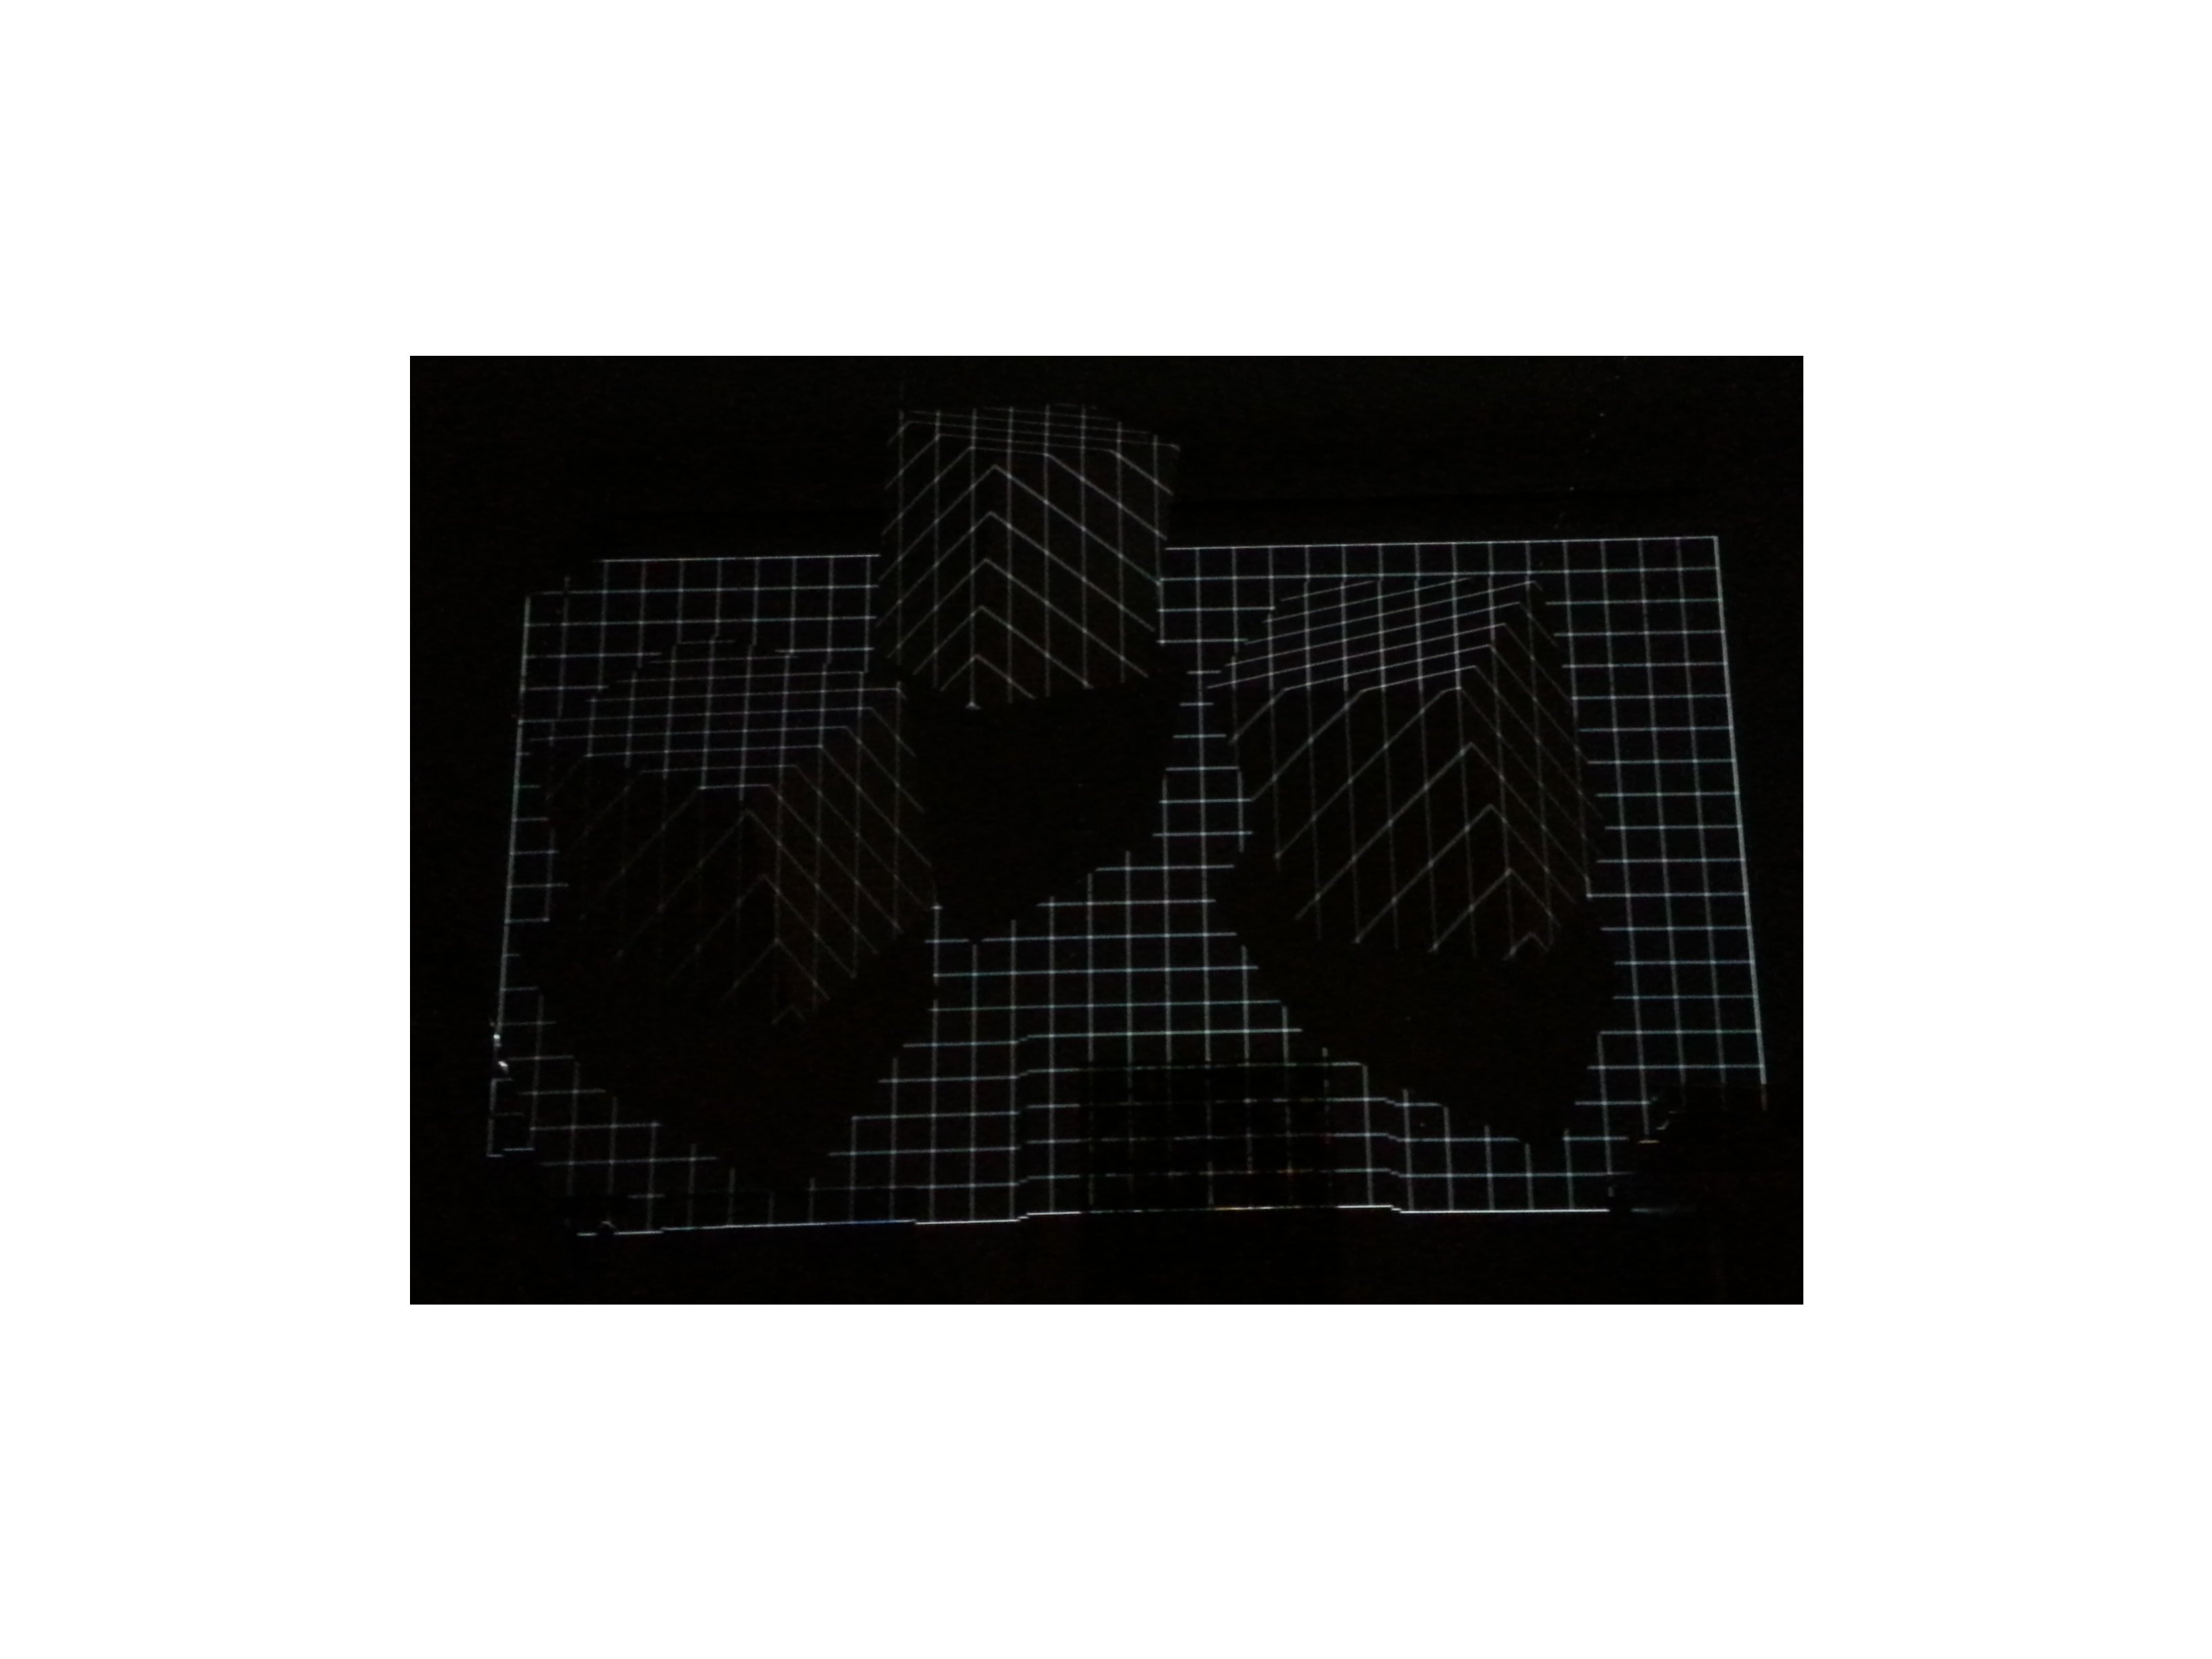
\includegraphics[width=0.9\textwidth]{./wuerfel_beamer}\\[0.3cm]   

\begin{wrapfigure}{r}{3cm} % l = Bild wird linksbündig positioniert, möglich ist auch r für rechtsbündig
% 8cm ist der Abstand von links, der für das Bild freigehalten wird, rechts davon kann Text stehen
\centering
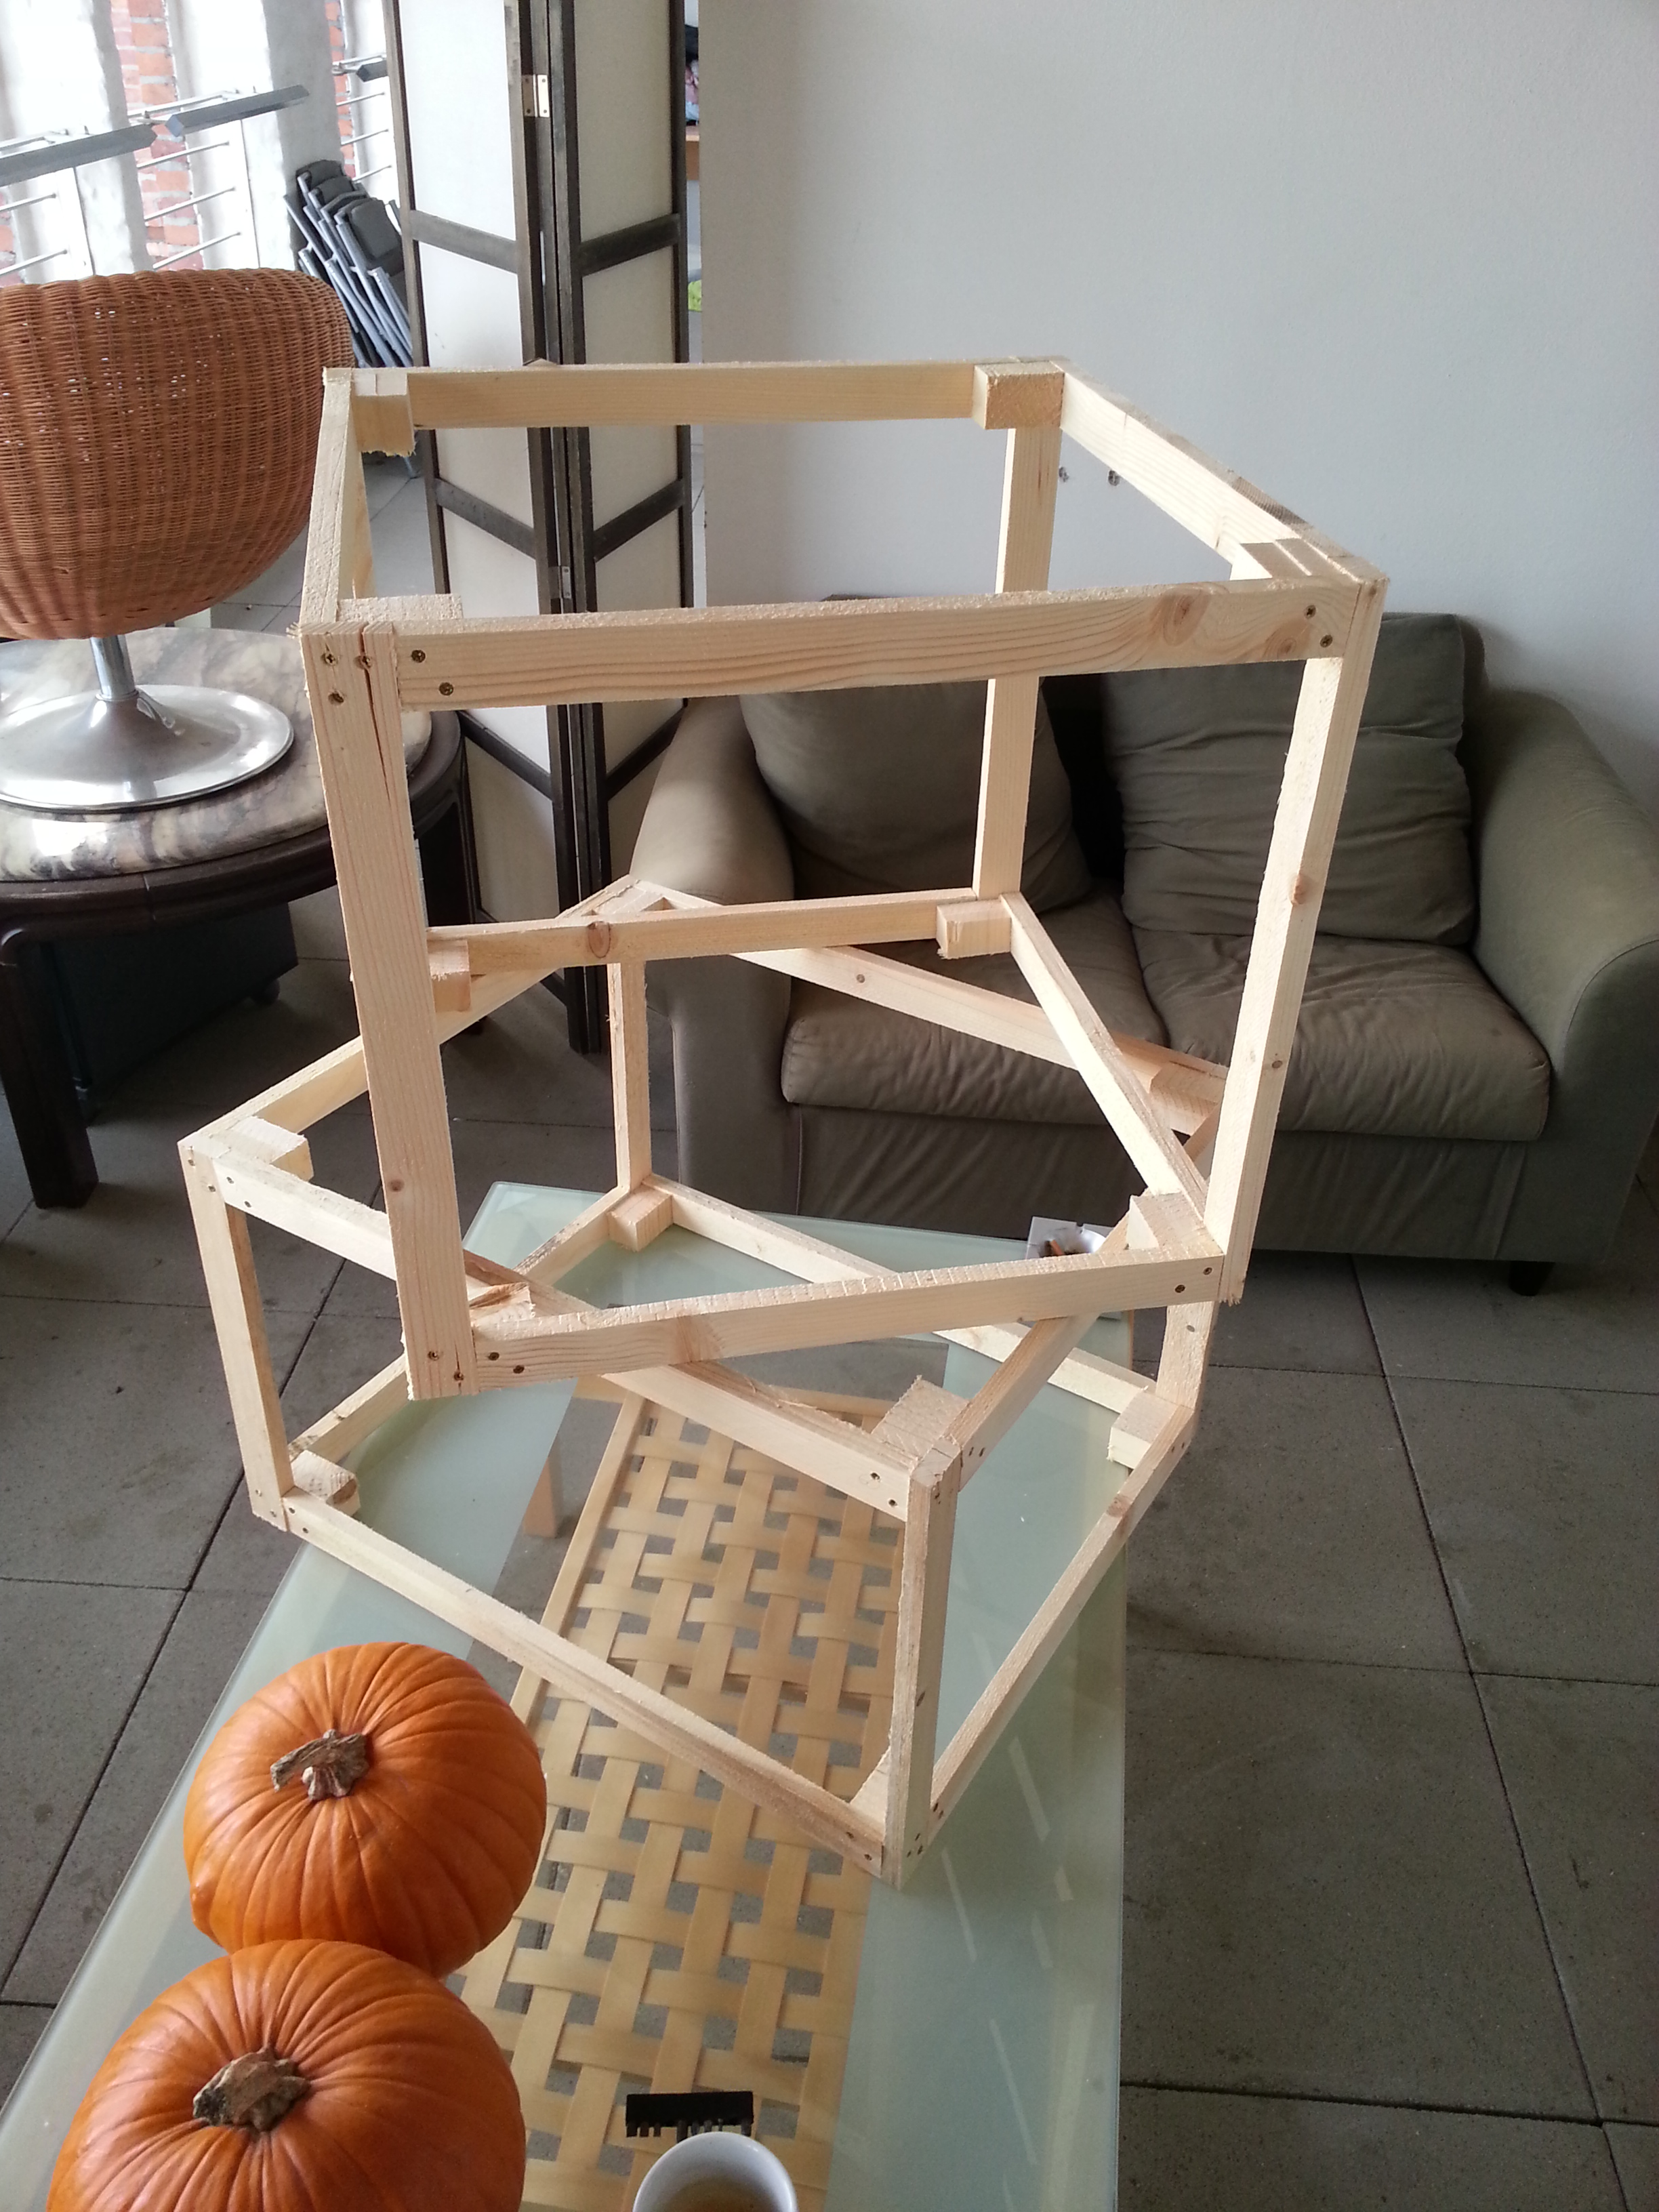
\includegraphics[width=0.4\textwidth]{./wuerfel_skelett}\\[0.3cm]   
\begin{flushright}
\textit{Würfelskelett}
\end{flushright}
\end{wrapfigure}
Das Würfelskelett bestehen aus dünnen 5x2cm dicken Holzlatten, die aneinander geschraubt sind.
Die Kanten der Würfel sind zwischen 35-50cm.  Die Projektionsflächen sind mit dicken Bastelpapier beklebt. Um die Würfel an die Decke zu hängen, wurde Packetband benutzt. hierbei wurden die Würfel direkt an der Decke an 2 Kanten Fixiert und noch einmal untereinander, um Schaukeln zu vermeiden.
Ein Beamer mit FullHD-Auflösung wurde für die Projektionen genutzt. Dabei war der Beamer ganz normal für eine Leinwand ausgerichtet und die Würfel wurden in das "Bild" reingehängt.Die Würfel wurden so ausgerichtete, dass eine Ecke zum Beamer zeigte, um die Projektionsflächen zu Maximieren.
Im oberen Bild sieht man die aufgehängten Würfel mit einem Testbild. 


\subsection{Die Software}
Um die Würfel anzusteuern wurde die Processing Bibliothek Surfacemapper verwendet. Mit dieser konnten wir mehrere Flächen erzeugen, sie auf die Seitenflächen der Würfel mappen und einzeln ansteuern. Anzumerken ist, dass die Software OpenGL nutzt um die Flächen zu verzerren. Dieses in Verbindung mit Processing kann sehr rechenintensiv sein und langsam, daher gab es  Optimierungsschwierigkeiten. Anbei sehen sie ein Bild mit den Würfeln wenn sie angestrahlt werden.
\\ \\
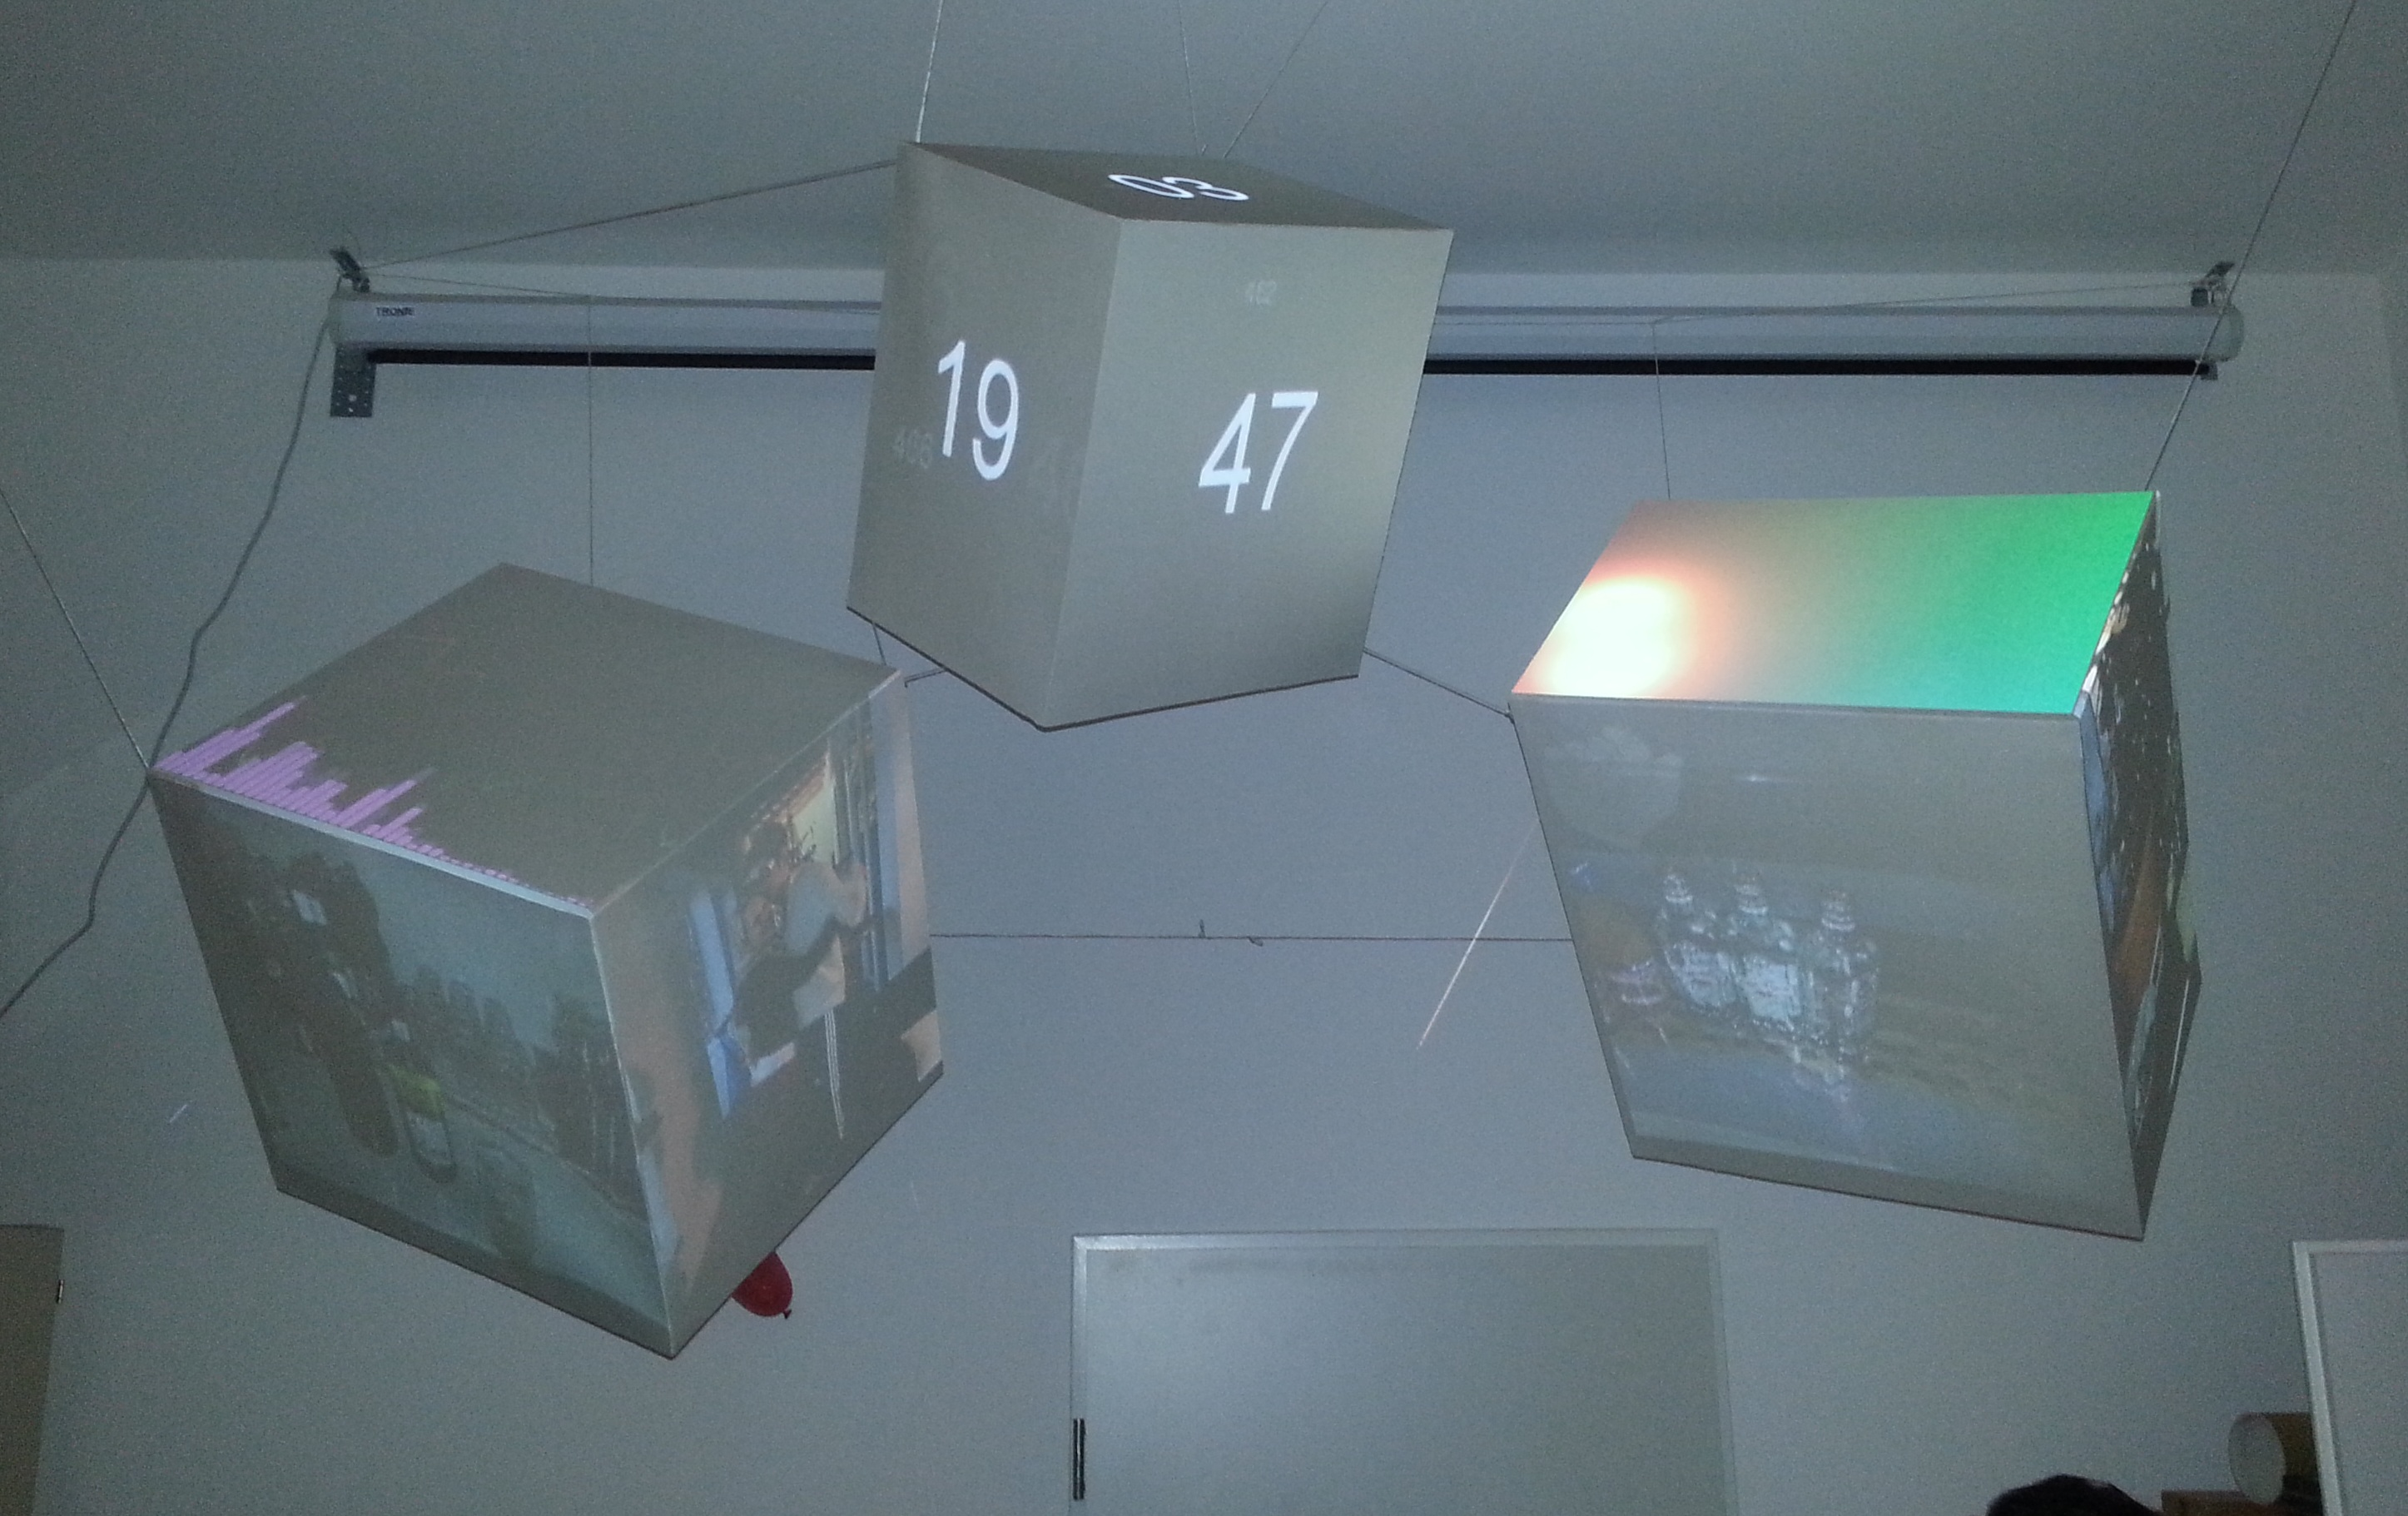
\includegraphics[width=0.7\textwidth]{./wuerfel_angestrahlt}\\[1cm]   
Die Bilder wurden ständig gewechselt. Neue Bilder die über eine Smartphone aufgenommen wurden, sind per DropBox in das System gekommen und wurden als nächstes angezeigt, ansonsten wurden zyklisch neue Bilder eingefadet. Zu große Bilder, wurden über die Flächen langsam geschoben. 
Der Countdown in der Mitte wurde nach 00 Uhr auf die Uhrzeit umgestellt. Links oben wurde eine FFT- in Waveform mit der aktuellen Musik angezeigt, rechts oben ein Effekt.
Wie schon erwähnt wurde auf den Würfeln angezeigt wenn die Türklingel betätigt wurde. Dafür nahm eine WebCam die in der Nähe der Türklingel installiert wurde die Meldeleuchte auf, und löste auf dem Hauptsystem einen Trigger aus.

\subsection{Aufwandsabschätzung}
Der Bau der Würfelt hat um die 30 Mannstunden in Anspruch genommen. Dabei ist besonders viel Zeit für Bekleben und das Ausrichten aufgewendet worden. Die Software hat rund 50 Mannstunden gekostet. Hierbei gabs einige Optimierungsschwierigkeiten mit OpenGL in Verbindung mit Processing.

\chapter{Konzepte mit Emitting Cubes}
\section{''Snake-around-the-Edge''}
\subsection{Ausgangspunkt}
Oftmals kommt es zu folgender Situation:\\
Man muss zum Amt um irgendeine Belanglosigkeit zu klären.\\
Aber bevor man mit jemandem dort sprechen kann um ihm zu erklären, dass man kein illegaler Einwanderer ist, sondern einfach jemand einen Accent in seinem Namen vergessen hat muss man warten.
Diese Wartezeit wird oft damti verbracht, Bücher zu lesen oder mit seinem Handy herumzuspielen - alleine...\\
...und hier kommen die Emitting Cubes ins Spiel!

\subsection{Die Idee und der Aufbau}
Um die Wartezeit an solchen Orten ein wenig zu verkürzen und zugleich, um für Gesellschaft bei der Tätigkeit des Herumsitzens zu schaffen, wurde ein Spiel nur für die Cubes entwickelt:\\
\\
\textbf{''Snake-around-the-Edge''}
\\\\
Ein Emitting Cube wird in der Mitte solcher Wartebereiche aufgehängt und von einem Beamer mit Spiegelsystem oder zwei Beamern von allen Seiten mittels Projection-Mapping angestrahlt.
Weiterhin existieren an mindestens sechs Plätzen kleine Tastaturen (es reichen hierbei Richtungs- und eine Start/Ende-Taste), die mit einem Stahlseil fest an dem jeweiligen Platz befestigt sind, um Diebstahl zu vermeiden.
Diese Tastaturen können per Funk mit dem Rechner, der den Beamer steuert, kommunizieren.

\subsection{Das Spiel}
Das Spielprinzip muss in einer solchen Umgebung natürlich einfach und jederzeit unterbrechbar sein.\\
Das Spielprinzip ist wie folgt:\\
\\
Man spielt eine Schlange, die Äpfel fressen muss. Sie bewegt sich automatisch in die Richtung weiter, die als letztes angewähklt wurde.
Es gibt auf dem Spielfeld eine bestimmte Anzahl Äpfel, die vom Rechner zufällig verteilt werden.
Wenn man einen Apfel frisst (sich darüber schlängelt) verschwindet der Apfel und irgendwo auf dem Spielfeld taucht ein neuer auf.
Außerdem wird die Schlange um ein bestimmtes Stück länger, wenn sie einen Apfel frisst.
Es gibt sonst nur zwei weitere Regeln: Die Schlange darf sich nicht selbst fressen und auch nicht eine Wand berühren.

\subsection{Umsetzung}
Das besondere an der Umsetzung mit dem Emitting Cube ist nun, dass sich das Spielfeld theoretisch über alle sechs Flächen des Würfels erstrecken kann.
Wenn eine Person das Spiel mit seinem Start-Button startet, wird es auf der ihm am nächsten gelegenen Fläche angezeigt.
Diese Fläche wird durch Triangulation mit mehreren Empfängern im Würfel bei der Kommunikation mit der Tastatur ermittelt.
Idealerweise hat eine Tastatur aber auch noch eine eindeutige Farbe, mit der die aktive Fläche jeweils leicht eingefärbt wird.
Nun kann dieser erste Spieler auf seiner Fläche spielen.
Dabei hat er allerdings die Einschränkung, dass die Fläche von Wänden umgeben ist.\\
\\
Möchte nun ein anderer Spieler mitspielen drückt er auf seiner Tastatur die Start-Taste.
Falls die ermittelte nächste Fläche an der des bereits spielenden anliegt, wird diese Wand nun bei beiden Spielern entfernt und sie können über die Würfelseite hinaus miteinander spielen.
Sobald der ''Kopf'' der Schlange die Würfelkante passiert, hat also der neue Spieler die Kontrolle und umgekehrt.
Dabei ist beim Design des Spiels darauf zu achten, dass neue Äpfel auf einer jeweils anderen Seite als der, 
auf der die Schlange sich gerade befindet, erzeugt werden, um zu verhindern, dass ein Spieler die ganze Zeit auf seiner Seite bleiben kann.

\subsection{Mehrfachnutzen}
Natürlich soll der Würfel auch informieren.
Daher ist geplant, dass beliebige Inhalte - also vom Betreiber aus vorgebbar - 
auf den restlichen Würfelflächen angezeigt, oder über Spielflächen mit einer gewissen Transparenz herübergelegt werden können.
Damit wird es möglich, dass der Betreiber Werbung schaltet oder die aktuellen Wartenummern auf allen Flächen des Würfels sichtbar sind.

\section{Perspektive-Buzzer}

\subsection{Ausgangspunkt Intention}
Eine Idee war es ein Spiel zu entwickeln was so einfach ist, dass es keine Erklärung brauch. Die Spieler sollten von selbst auf die Regeln kommen und das Spiel entdecken.
Hierbei sollen die Spieler abwechselnd die Buzzer betätigen um im Spiel voranzukommen. Die Folge der Bazzer-Drücke sollte auf den Cubes angezeigt werden sowie die erreichten Spielzüge in Folge. Im Laufe des Spiels verkürzen sich die Intervalle zwischen den Bazzer-Hits und es wird schwieriger mitzukommen. Der besondere Faktor kommt in der Darstellung der Bazzer auf den Cubes. Neben/unter den Bazzer müssen Kameras installiert sein, die eine Aufnahmen aus der Ameisenperspektive machen, d.h. wenn keine Spieler im Bild ist und direkt drauf guckt, Zeigt jede Kamera nur die Decke, und ist somit nicht unterscheidbar. Erst wenn ein Spieler ins Bild tritt wird der nächste Spielzug ersichtlich. Dadurch entdeckt der Spieler ziemlich schnell, wie das Spiel gespielt werden muss. Die Intention ist es, dass irgendwann mehr Spieler an dem Spiel beteiligt werden da ein Spieler zwischen den Buzzern hin und her laufen muss, nur dann kann das Spiel länger gespielt werden.

\subsection{Idee und Aufbau}
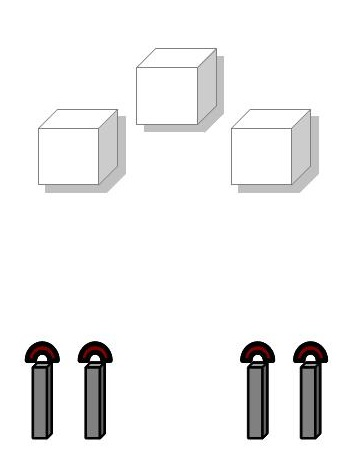
\includegraphics[width=0.5\textwidth]{./perspektiv}\\[0.3cm]   
\\
Vor 3 Würfeln sollen je 2x2 Buzzer-Paare im Raum stehen. Der Raum braucht viel Fläche und solle möglichst eine einheitlich weisse Decke besitzen. Die Würfel werden von der gegenüberliegenden Wand mit einem Beamer angestrahlt. Dabei werden 7 Flächen angestrahlt, 3 von dem mittleren Würfel und jeweils 2 von den seitlichen Würfeln. Die Buzzer haben jeweils eine Kamera die nach oben gerichtet ist und stehen auf hüfthohen Podesten.

\subsection{Das Spiel}
Ziel des Spiels ist es 2 Buzzer hintereinander in der vorgegebenen Zeit zu drücken. Hierfür wird auf den unteren Flächen des linken und rechten Würfels das Bild der Buzzer-Kamera eingeblendet welcher als nächstes gedrückt werden muss, die oberen Flächen zeigen einen Countdown, wieviel Zeit noch übrig ist den Buzzer zu drücken, bis das Spiel abgebrochen wird.  Auf der linken und rechten Fläche des mittleren Würfels wird immer jeweilige nächste Buzzer gezeigt, der in der nächsten Runde gedrückt werden muss. Die Obere Fläche zeigt die Zahl der erfolgreich abgeschlossenen Runden. 
Jede Runde begint also damit das die Kamerabilder der Flächen die als nächsten gedrückt werden müssen vom den linken und rechten Seiten des mittleren Würfel auf den linken bzw. rechten würfel springen und ein Countdown auf diesen würfeln angezeigt wird. Während diese Countdowns hat man die Möglichkeit die passenden Buzzer zu suchen um ihn zu drücken und eine neue Runde zu beginnen. Es müssen immer 2 Buzzer pro Runde gedrückt werden. Sobald ein richtiger Buzzer gedrückt wird, wird eine Momentaufnahme der Kamera gezeigt und der Countdown für den jeweiligen Würfel gestoppt. Der ander Countdown für den 2. Buzzer läuft weiter und muss vor Ablauf gestoppt werde. Dabei wird der Countdown von Runde zu Runde leicht verringert. Schnell hat man nur dir Möglichkeit das Spiel zu spielen, wenn man sich zu mehreren zusammen tut und an die Buzzer in die Kamera stellt.

\subsection{Umsetztung}
Die Würfel sind wie schon im ersten Kapitel beschrieben gebaut und die Software dafür leicht zu modifizieren. Die Buzzer müssen hüfthoch auf kleinen Podesten im Raum verteilt sein. Dabei sollen 2 möglichst nah beeinander stehen um die von einer Person bedient zu werden. Die Kameras in den Buzzern sind an die Decke gerichtet und senden ihr Bild an das System mit der Projektionssoftware. Über ein Arduino-Board können die genutzten Buzzer und die Projektionssoftware kommunizieren.

Für die Software wird weiterhin Java und Processing genutzt mit OpenGL und dem Plugin Surfacemapper.
Mit dem Plugin Surfacemapper, können auch Kameraaufnahmen auf die Projektionsflächen geworfen werden.


\end{document}






